\documentclass{ieeeaccess}
\usepackage{cite}
\usepackage{amsmath,amssymb,amsfonts}
\usepackage{algorithmic}
\usepackage{graphicx}
\usepackage{textcomp}
\usepackage{threeparttable}

\usepackage{bm}
\makeatletter
\AtBeginDocument{\DeclareMathVersion{bold}
\SetSymbolFont{operators}{bold}{T1}{times}{b}{n}
\SetSymbolFont{NewLetters}{bold}{T1}{times}{b}{it}
\SetMathAlphabet{\mathrm}{bold}{T1}{times}{b}{n}
\SetMathAlphabet{\mathit}{bold}{T1}{times}{b}{it}
\SetMathAlphabet{\mathbf}{bold}{T1}{times}{b}{n}
\SetMathAlphabet{\mathtt}{bold}{OT1}{pcr}{b}{n}
\SetSymbolFont{symbols}{bold}{OMS}{cmsy}{b}{n}
\renewcommand\boldmath{\@nomath\boldmath\mathversion{bold}}}
\makeatother

\def\BibTeX{{\rm B\kern-.05em{\sc i\kern-.025em b}\kern-.08em
    T\kern-.1667em\lower.7ex\hbox{E}\kern-.125emX}}

%Your document starts from here ___________________________________________________
\begin{document}
\history{Date of publication xxxx 00, 0000, date of current version xxxx 00, 0000.}
\doi{10.1109/ACCESS.2024.0429000}

\title{Studying the Effects of Water to Cement Ratio on the Mechanical Properties of 
       Concrete}
\author{
    \uppercase{Pranav V}\authorrefmark{1}, \uppercase{Abhay V}\authorrefmark{1}, 
    \uppercase{Suyash J}\authorrefmark{1}, \uppercase{Soham S}\authorrefmark{2},
    \uppercase{Rakshith P}\authorrefmark{3}
}

\address[1]{Department of Electronics and Communication Engineering,
            RV College of Engineering, Bangalore, India}
\address[1]{Department of Mechanical Engineering,
            RV College of Engineering, Bangalore, India}
\address[1]{Department of Information Science and Engineering,
            RV College of Engineering, Bangalore, India}

\markboth
{Author \headeretal: Preparation of Papers for IEEE TRANSACTIONS and JOURNALS}
{Author \headeretal: Preparation of Papers for IEEE TRANSACTIONS and JOURNALS}

\corresp{Corresponding author: Pranav V (e-mail: pranavvv.ec24@rvce.edu.in).}


\begin{abstract}
Pervious concrete is a sustainable construction material developed to mitigate
urban issues such as stormwater runoff, reduced groundwater recharge, and
surface flooding. This study focuses on the design and experimental
evaluation of a pervious concrete mix aimed at achieving adequate
mechanical strength while ensuring desirable permeability. The
investigation involved selecting suitable aggregates, determining an
appropriate water–cement ratio, and incorporating admixtures to enhance
overall performance. Compressive strength, tensile strength, and
permeability tests were conducted to assess the mix’s applicability in
pavements and low-traffic areas. The results demonstrated that the proposed
mix design offers a practical balance between structural integrity and
permeability, highlighting its potential as an environmentally friendly
alternative to conventional paving materials. Additionally, the paper
discusses challenges encountered during mix design and implementation and
suggests directions for future research to enable its effective use in
large-scale applications.
\end{abstract}

\begin{keywords}
    Pervious concrete
\end{keywords}

\titlepgskip=-21pt

\maketitle

\section{Introduction}
\label{sec:introduction}
\PARstart{R}{apid} urbanization has led to extensive construction of impervious 
surfaces such as asphalt and conventional concrete pavements, which disrupt the 
natural hydrological cycle. These surfaces prevent water infiltration, resulting 
in increased surface runoff, urban flooding, and reduced groundwater recharge. 
In response to these environmental concerns, there has been a growing interest 
in sustainable construction materials that support stormwater management. One 
such material is pervious concrete, a special type of concrete with a high void 
content that allows water to pass through its structure. 

Pervious concrete is composed of coarse aggregates, cement, water, and little to 
no fine aggregates. Its interconnected pore network enables infiltration of 
rainwater, making it suitable for sidewalks, parking lots, driveways, and 
low-traffic roads. In addition to hydrological benefits, pervious concrete can 
reduce the urban heat island effect, improve skid resistance, and contribute 
toward LEED (Leadership in Energy and Environmental Design) credits in green 
building certification systems. 

Despite its advantages, the widespread use of pervious concrete has been limited 
due to challenges in achieving an optimal balance between permeability and 
mechanical strength. In this study, we focus on the effects of the  water-cement 
ratio on the physical properties of pervious concrete. To this end, two batches 
of 6 pervious concrete cylinders, with the second batch having a lower 
water-cement ratio, were made, and tested for compresssive strength, split 
tensile strength, and permeability. Superplasticizer (SP) was used to increase 
the workability of the mixes made with the second recipe. 



\section{Experimental Setup}
Two batches of 6 cylinders each were cast. Common to both batches were the
cementitious material which was a mixture of cement and fly-ash in the ratio of 
4:1 by mass, coarse aggregates whose sizes ranged from 4.75-9.5 mm, 
and polypropylene fibres (PPF). 
\
\begin{table}
    \begin{threeparttable}
        \caption{\textbf{Mix Design}}
        \label{table:mix-design}
        \setlength{\tabcolsep}{20pt}
        \def\arraystretch{1.5}%
        \begin{tabular}{ l r  r }
            \hline
            & \multicolumn{1}{c}{Batch 1} & \multicolumn{1}{c}{Batch 2} \\
            \hline
            Cement, $kg/m\textsuperscript{3}$  & 280  & 280  \\
            Coarse Aggregate, $kg/m\textsuperscript{3}$ & 1420 & 1420 \\
            Fly-ash, $kg/m\textsuperscript{3}$ & 70   & 70   \\
            Water, $kg/m\textsuperscript{3}$   & 119  & 95.2 \\
            SP, $\%$\textsuperscript{1}        & ---  & 0.5  \\
            PPF, $\%$\textsuperscript{2}       & 0.2  & 0.2  \\
            \hline
        \end{tabular} 
        \begin{tablenotes}
            \item[1] \footnotesize of cementitious material
            \item[2] \footnotesize of aggregates
        \end{tablenotes}
    \end{threeparttable}
\end{table}
\
The rest of the ingredients are given in table \ref{table:mix-design}.

\section{Testing Method}
The samples were tested after 14 and 28 days for tensile and compressive 
strenghts, and after 28 days for permeability.

\subsection{Compressive Strength}
The sample was placed in the universal testing machine (UTM) on one of its 
circular faces, and compressed. The pace rate was set to 1.8 KN/s. 
The compressive strength $f_c$ is calculated with the formula 
\[f_c = \frac{P}{A}\] where $P$ is the maximum force on the sample, and $A$ is
the area over which the force is applied.

\subsection{Tensile Strength}
The tensile strength was found using the Brazilian test, in which, the sample
was placed horizontally, in between two metal bars oriented parallel to the axis
of the sample, inside the UTM. The tensile strength $f_t$ was calculated with
the formula \[f_t = \frac{2P}{\pi LD}\] where $P$ is the force at the point of
failure, and $L$ and $D$ are respectively the length and the diameter of the
sample.

\subsection{Permeability}
The tensile strength was found using a makeshift falling head permeameter.
By measuring the time taken for the head to move from a height $h_1$ down to
$h_2$, the permeability $k$ can be calculated using the formula 
\[k = \frac{aL}{At} \ln{\frac{h_1}{h_2}}\] where $a$ is the cross-sectional area
of the standpipe, $t$ is the time taken for the head to fall from $h_1$ to 
$h-2$, and $L$ and $A$ are the dimensions of the sample.


\section{Results}

\begin{table}[h]
    \begin{threeparttable}
        \caption{\textbf{Compressive and Tensile Strength}}
        \label{table:str-test}
        \setlength{\tabcolsep}{16.5pt}
        \def\arraystretch{1.5}%
        \begin{tabular}{ l r r r r }
            \hline
            & \multicolumn{2}{c}{Compressive, $Mpa$} & 
                \multicolumn{2}{c}{Tensile, $Mpa$} \\

            \cline{2-5}
            & \multicolumn{1}{c}{14} & \multicolumn{1}{c}{28} & 
                \multicolumn{1}{c}{14} & \multicolumn{1}{c}{28} \\

            \hline

            Batch 1 & 5.62 & 7.49  & 0.71 & 0.85 \\
            Batch 2 & 8.02 & 10.08 & 1.15 & 1.33 \\

            \hline
        \end{tabular} 
        \begin{tablenotes}
            \item Results of the compressive and tensile tests at the end of 
            14 and 28 days of curing.
        \end{tablenotes}
    \end{threeparttable}
\end{table}

\begin{table}[h]
    \begin{threeparttable}
        \caption{\textbf{Permeability}}
        \label{table:perm-test}
        \setlength{\tabcolsep}{16.5pt}
        \def\arraystretch{1.5}%
        \begin{tabular}{ l r r }
            \hline
            & \multicolumn{1}{c}{14} & \multicolumn{1}{c}{28} \\
            \hline

            Batch 1 & 2.90 & 1.73 \\ 
            Batch 2 & 1.93 & 1.15 \\

            \hline
        \end{tabular} 
        \begin{tablenotes}
            \item Results of the permeability tests at the end of 
            14 and 28 days of curing.
        \end{tablenotes}
    \end{threeparttable}
\end{table}

From the results, given by table \ref{table:str-test}, it is apparent that the 
amount of water used in the mix greatly affects the final strength of the 
concrete, with the ones having a lower water-cement ratio outperforming the ones 
with a higher water-cement ratio.


\section{Conclusion}
Although a conclusion may review the  main points of the paper, do not replicate the abstract as the conclusion. A
conclusion might elaborate on the importance of the work or suggest
applications and extensions.

If you have multiple appendices, use the $\backslash$appendices command below. If you have only one appendix, use
$\backslash$appendix[Appendix Title]

\appendices
\section{\break Footnotes}
Number footnotes separately in superscript numbers.\footnote{It is recommended that footnotes be avoided (except for
the unnumbered footnote with the receipt date on the first page). Instead,
try to integrate the footnote information into the text.} Place the actual
footnote at the bottom of the column in which it is cited; do not put
footnotes in the reference list (endnotes). Use letters for table footnotes
(see Table \ref{table}).

\section{\break Submitting Your Paper for Review}

\subsection{Final Stage}
When your article is accepted, you can submit the final files, including figures, tables, and photos, per the journal's guidelines through the submission system used to submit the articlle.
 You may use \emph{Zip} for large files, or compress files using \emph{Compress, Pkzip, Stuffit,} or \emph{Gzip.}

In addition, designate one author as the ``corresponding author.'' This is the author to
whom proofs of the paper will be sent. Proofs are sent to the corresponding
author only.

\subsection{Review Stage Using IEEE Author Portal}
Article contributions to IEEE Access should be submitted electronically on the IEEE Author Portal. For more information, please visit
\underline{https://ieeeaccess.ieee.org/}.

Along with other information, you will be asked to select the subject from a
pull-down list. There are various steps to the
submission process; you must complete all steps for a complete submission.
At the end of each step you must click ``Save and Continue''; just uploading
the paper is not sufficient. After the last step, you should see a
confirmation that the submission is complete. You should also receive an
e-mail confirmation. For inquiries regarding the submission of your article, please contact ieeeaccess@ieee.org.

The manuscript should be prepared in a double column, single-spaced format using a required IEEE Access template.
A Word or LaTeX file and a PDF file are both required upon submission in the IEEE Author Portal.

\subsection{Final Stage Using IEEE Author Portal}
Upon acceptance, you will receive an email with specific instructions

Designate the author who submitted the manuscript on
IEEE Author Portal as the ``corresponding author.'' This is the only
author to whom proofs of the paper will be sent.

\subsection{Copyright Form}
Authors must submit an electronic IEEE Copyright Form (eCF) upon submitting
their final manuscript files. You can access the eCF system through your
manuscript submission system or through the Author Gateway. You are
responsible for obtaining any necessary approvals and/or security
clearances. For additional information on intellectual property rights,
visit the IEEE Intellectual Property Rights department web page at
\underline{http://www.ieee.org/publications\_standards/publications/}\break\underline{rights/index.html}.

\section{\break IEEE Publishing Policy}
The general IEEE policy requires that authors should only submit original
work that has neither appeared elsewhere for publication, nor is under
review for another refereed publication. The submitting author must disclose
all prior publication(s) and current submissions when submitting a
manuscript. Do not publish ``preliminary'' data or results. To avoid any delays in
publication, please be sure to follow these instructions.  Final
submissions should include source files of your accepted manuscript, high
quality graphic files, and a formatted pdf file. If you have any questions
regarding the final submission process, please contact the administrative
contact for the journal.
author is responsible for obtaining agreement of all coauthors and any
consent required from employers or sponsors before submitting an article.

The IEEE Access Editorial Office does not publish conference
records or proceedings, but can publish articles related to conferences that
have undergone rigorous peer review. Minimally, two reviews are required for
every article submitted for peer review.

\section{\break Publication Principles}
Authors should consider the following points:

\begin{enumerate}
\item Technical papers submitted for publication must advance the state of knowledge and must cite relevant prior work.
\item The length of a submitted paper should be commensurate with the importance, or appropriate to the complexity, of the work. For example, an obvious extension of previously published work might not be appropriate for publication or might be adequately treated in just a few pages.
\item Authors must convince both peer reviewers and the editors of the scientific and technical merit of a paper; the standards of proof are higher when extraordinary or unexpected results are reported.
\item Because replication is required for scientific progress, papers submitted for publication must provide sufficient information to allow readers to perform similar experiments or calculations and
use the reported results. Although not everything need be disclosed, a paper
must contain new, useable, and fully described information. For example, a
specimen's chemical composition need not be reported if the main purpose of
a paper is to introduce a new measurement technique. Authors should expect
to be challenged by reviewers if the results are not supported by adequate
data and critical details.
\item Papers that describe ongoing work or announce the latest technical achievement, which are suitable for presentation at a professional conference, may not be appropriate for publication.
\end{enumerate}



\section{\break Reference Examples}

\begin{itemize}

\item \emph{Basic format for books:}\\
J. K. Author, ``Title of chapter in the book,'' in \emph{Title of His Published Book, x}th ed. City of Publisher, (only U.S. State), Country: Abbrev. of Publisher, year, ch. $x$, sec. $x$, pp. \emph{xxx--xxx.}\\
See \cite{b1,b2}.

\item \emph{Basic format for periodicals:}\\
J. K. Author, ``Name of paper,'' \emph{Abbrev. Title of Periodical}, vol. \emph{x, no}. $x, $pp\emph{. xxx--xxx, }Abbrev. Month, year, DOI. 10.1109.\emph{XXX}.123456.\\
See \cite{b3}--\cite{b5}.

\item \emph{Basic format for reports:}\\
J. K. Author, ``Title of report,'' Abbrev. Name of Co., City of Co., Abbrev. State, Country, Rep. \emph{xxx}, year.\\
See \cite{b6,b7}.

\item \emph{Basic format for handbooks:}\\
\emph{Name of Manual/Handbook, x} ed., Abbrev. Name of Co., City of Co., Abbrev. State, Country, year, pp. \emph{xxx--xxx.}\\
See \cite{b8,b9}.

\item \emph{Basic format for books (when available online):}\\
J. K. Author, ``Title of chapter in the book,'' in \emph{Title of
Published Book}, $x$th ed. City of Publisher, State, Country: Abbrev.
of Publisher, year, ch. $x$, sec. $x$, pp. \emph{xxx--xxx}. [Online].
Available: \underline{http://www.web.com}\\
See \cite{b10}--\cite{b13}.

\item \emph{Basic format for journals (when available online):}\\
J. K. Author, ``Name of paper,'' \emph{Abbrev. Title of Periodical}, vol. $x$, no. $x$, pp. \emph{xxx--xxx}, Abbrev. Month, year. Accessed on: Month, Day, year, DOI: 10.1109.\emph{XXX}.123456, [Online].\\
See \cite{b14}--\cite{b16}.

\item \emph{Basic format for papers presented at conferences (when available online): }\\
J.K. Author. (year, month). Title. presented at abbrev. conference title. [Type of Medium]. Available: site/path/file\\
See \cite{b17}.

\item \emph{Basic format for reports and handbooks (when available online):}\\
J. K. Author. ``Title of report,'' Company. City, State, Country. Rep. no., (optional: vol./issue), Date. [Online] Available: site/path/file\\
See \cite{b18,b19}.

\item \emph{Basic format for computer programs and electronic documents (when available online): }\\
Legislative body. Number of Congress, Session. (year, month day). \emph{Number of bill or resolution}, \emph{Title}. [Type of medium]. Available: site/path/file\\
See \cite{b20}.

\item \emph{Basic format for patents (when available online):}\\
Name of the invention, by inventor's name. (year, month day). Patent Number [Type of medium]. Available: site/path/file\\
See \cite{b21}.

\item \emph{Basic format}\emph{for conference proceedings (published):}\\
J. K. Author, ``Title of paper,'' in \emph{Abbreviated Name of Conf.}, City of Conf., Abbrev. State (if given), Country, year, pp. \emph{xxxxxx.}\\
See \cite{b22}.

\item \emph{Example for papers presented at conferences (unpublished):}\\
See \cite{b23}.

\item \emph{Basic format for patents}$:$\\
J. K. Author, ``Title of patent,'' U.S. Patent \emph{x xxx xxx}, Abbrev. Month, day, year.\\
See \cite{b24}.

\item \emph{Basic format for theses (M.S.) and dissertations (Ph.D.):}
\begin{enumerate}
\item J. K. Author, ``Title of thesis,'' M.S. thesis, Abbrev. Dept., Abbrev. Univ., City of Univ., Abbrev. State, year.
\item J. K. Author, ``Title of dissertation,'' Ph.D. dissertation, Abbrev. Dept., Abbrev. Univ., City of Univ., Abbrev. State, year.
\end{enumerate}
See \cite{b25,b26}.

\item \emph{Basic format for the most common types of unpublished references:}
\begin{enumerate}
\item J. K. Author, private communication, Abbrev. Month, year.
\item J. K. Author, ``Title of paper,'' unpublished.
\item J. K. Author, ``Title of paper,'' to be published.
\end{enumerate}
See \cite{b27}--\cite{b29}.

\item \emph{Basic formats for standards:}
\begin{enumerate}
\item \emph{Title of Standard}, Standard number, date.
\item \emph{Title of Standard}, Standard number, Corporate author, location, date.
\end{enumerate}
See \cite{b30,b31}.

\item \emph{Article number in~reference examples:}\\
See \cite{b32,b33}.

\item \emph{Example when using et al.:}\\
See \cite{b34}.

\end{itemize}


\section*{Acknowledgment}
The preferred spelling of the word ``acknowledgment'' in American English is
without an ``e'' after the ``g.'' Use the singular heading even if you have
many acknowledgments. Avoid expressions such as ``One of us (S.B.A.) would
like to thank $\ldots$ .'' Instead, write ``F. A. Author thanks $\ldots$ .'' In most
cases, sponsor and financial support acknowledgments are placed in the
unnumbered footnote on the first page, not here.


\begin{thebibliography}{00}

\bibitem{b1} G. O. Young, ``Synthetic structure of industrial plastics,'' in \emph{Plastics,} 2\textsuperscript{nd} ed., vol. 3, J. Peters, Ed. New York, NY, USA: McGraw-Hill, 1964, pp. 15--64.

\bibitem{b2} W.-K. Chen, \emph{Linear Networks and Systems.} Belmont, CA, USA: Wadsworth, 1993, pp. 123--135.

\bibitem{b3} J. U. Duncombe, ``Infrared navigation---Part I: An assessment of feasibility,'' \emph{IEEE Trans. Electron Devices}, vol. ED-11, no. 1, pp. 34--39, Jan. 1959, 10.1109/TED.2016.2628402.

\bibitem{b4} E. P. Wigner, ``Theory of traveling-wave optical laser,'' \emph{Phys. Rev}., vol. 134, pp. A635--A646, Dec. 1965.

\bibitem{b5} E. H. Miller, ``A note on reflector arrays,'' \emph{IEEE Trans. Antennas Propagat}., to be published.

\bibitem{b6} E. E. Reber, R. L. Michell, and C. J. Carter, ``Oxygen absorption in the earth's atmosphere,'' Aerospace Corp., Los Angeles, CA, USA, Tech. Rep. TR-0200 (4230-46)-3, Nov. 1988.

\bibitem{b7} J. H. Davis and J. R. Cogdell, ``Calibration program for the 16-foot antenna,'' Elect. Eng. Res. Lab., Univ. Texas, Austin, TX, USA, Tech. Memo. NGL-006-69-3, Nov. 15, 1987.

\bibitem{b8} \emph{Transmission Systems for Communications}, 3\textsuperscript{rd} ed., Western Electric Co., Winston-Salem, NC, USA, 1985, pp. 44--60.

\bibitem{b9} \emph{Motorola Semiconductor Data Manual}, Motorola Semiconductor Products Inc., Phoenix, AZ, USA, 1989.

\bibitem{b10} G. O. Young, ``Synthetic structure of industrial
plastics,'' in Plastics, vol. 3, Polymers of Hexadromicon, J. Peters,
Ed., 2\textsuperscript{nd} ed. New York, NY, USA: McGraw-Hill, 1964, pp. 15-64.
[Online]. Available:
\underline{http://www.bookref.com}.

\bibitem{b11} \emph{The Founders' Constitution}, Philip B. Kurland
and Ralph Lerner, eds., Chicago, IL, USA: Univ. Chicago Press, 1987.
[Online]. Available: \underline{http://press-pubs.uchicago.edu/founders/}

\bibitem{b12} The Terahertz Wave eBook. ZOmega Terahertz Corp., 2014.
[Online]. Available:
\underline{http://dl.z-thz.com/eBook/zomegaebookpdf\_1206\_sr.pdf}. Accessed on: May 19, 2014.

\bibitem{b13} Philip B. Kurland and Ralph Lerner, eds., \emph{The
Founders' Constitution.} Chicago, IL, USA: Univ. of Chicago Press,
1987, Accessed on: Feb. 28, 2010, [Online] Available:
\underline{http://press-pubs.uchicago.edu/founders/}

\bibitem{b14} J. S. Turner, ``New directions in communications,'' \emph{IEEE J. Sel. Areas Commun}., vol. 13, no. 1, pp. 11-23, Jan. 1995.

\bibitem{b15} W. P. Risk, G. S. Kino, and H. J. Shaw, ``Fiber-optic frequency shifter using a surface acoustic wave incident at an oblique angle,'' \emph{Opt. Lett.}, vol. 11, no. 2, pp. 115--117, Feb. 1986.

\bibitem{b16} P. Kopyt \emph{et al., ``}Electric properties of graphene-based conductive layers from DC up to terahertz range,'' \emph{IEEE THz Sci. Technol.,} to be published. DOI: 10.1109/TTHZ.2016.2544142.

\bibitem{b17} PROCESS Corporation, Boston, MA, USA. Intranets:
Internet technologies deployed behind the firewall for corporate
productivity. Presented at INET96 Annual Meeting. [Online].
Available: \underline{http://home.process.com/Intranets/wp2.htp}

\bibitem{b18} R. J. Hijmans and J. van Etten, ``Raster: Geographic analysis and modeling with raster data,'' R Package Version 2.0-12, Jan. 12, 2012. [Online]. Available: \underline {http://CRAN.R-project.org/package=raster}

\bibitem{b19} Teralyzer. Lytera UG, Kirchhain, Germany [Online].
Available:
\underline{http://www.lytera.de/Terahertz\_THz\_Spectroscopy.php?id=home}, Accessed on: Jun. 5, 2014.

\bibitem{b20} U.S. House. 102\textsuperscript{nd} Congress, 1\textsuperscript{st} Session. (1991, Jan. 11). \emph{H. Con. Res. 1, Sense of the Congress on Approval of}  \emph{Military Action}. [Online]. Available: LEXIS Library: GENFED File: BILLS

\bibitem{b21} Musical toothbrush with mirror, by L.M.R. Brooks. (1992, May 19). Patent D 326 189 [Online]. Available: NEXIS Library: LEXPAT File: DES

\bibitem{b22} D. B. Payne and J. R. Stern, ``Wavelength-switched pas- sively coupled single-mode optical network,'' in \emph{Proc. IOOC-ECOC,} Boston, MA, USA, 1985, pp. 585--590.

\bibitem{b23} D. Ebehard and E. Voges, ``Digital single sideband detection for interferometric sensors,'' presented at the \emph{2\textsuperscript{nd} Int. Conf. Optical Fiber Sensors,} Stuttgart, Germany, Jan. 2-5, 1984.

\bibitem{b24} G. Brandli and M. Dick, ``Alternating current fed power supply,'' U.S. Patent 4 084 217, Nov. 4, 1978.

\bibitem{b25} J. O. Williams, ``Narrow-band analyzer,'' Ph.D. dissertation, Dept. Elect. Eng., Harvard Univ., Cambridge, MA, USA, 1993.

\bibitem{b26} N. Kawasaki, ``Parametric study of thermal and chemical nonequilibrium nozzle flow,'' M.S. thesis, Dept. Electron. Eng., Osaka Univ., Osaka, Japan, 1993.

\bibitem{b27} A. Harrison, private communication, May 1995.

\bibitem{b28} B. Smith, ``An approach to graphs of linear forms,'' unpublished.

\bibitem{b29} A. Brahms, ``Representation error for real numbers in binary computer arithmetic,'' IEEE Computer Group Repository, Paper R-67-85.

\bibitem{b30} IEEE Criteria for Class IE Electric Systems, IEEE Standard 308, 1969.

\bibitem{b31} Letter Symbols for Quantities, ANSI Standard Y10.5-1968.

\bibitem{b32} R. Fardel, M. Nagel, F. Nuesch, T. Lippert, and A. Wokaun, ``Fabrication of organic light emitting diode pixels by laser-assisted forward transfer,'' \emph{Appl. Phys. Lett.}, vol. 91, no. 6, Aug. 2007, Art. no. 061103.~

\bibitem{b33} J. Zhang and N. Tansu, ``Optical gain and laser characteristics of InGaN quantum wells on ternary InGaN substrates,'' \emph{IEEE Photon. J.}, vol. 5, no. 2, Apr. 2013, Art. no. 2600111

\bibitem{b34} S. Azodolmolky~\emph{et al.}, Experimental demonstration of an impairment aware network planning and operation tool for transparent/translucent optical networks,''~\emph{J. Lightw. Technol.}, vol. 29, no. 4, pp. 439--448, Sep. 2011.

\end{thebibliography}

\begin{IEEEbiography}[{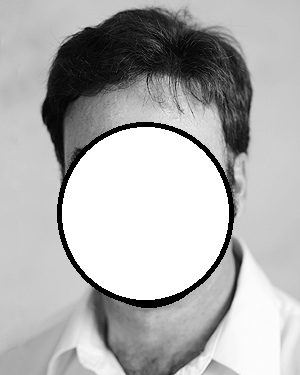
\includegraphics[width=1in,height=1.25in,clip,keepaspectratio]{author1.png}}]{First A. Author} received the B.S. and M.S. degrees in aerospace engineering from
the University of Virginia, Charlottesville, in 2001 and the Ph.D. degree in
mechanical engineering from Drexel University, Philadelphia, PA, in 2008.

From 2001 to 2004, he was a Research Assistant with the Princeton Plasma
Physics Laboratory. Since 2009, he has been an Assistant Professor with the
Mechanical Engineering Department, Texas A{\&}M University, College Station.
He is the author of three books, more than 150 articles, and more than 70
inventions. His research interests include high-pressure and high-density
nonthermal plasma discharge processes and applications, microscale plasma
discharges, discharges in liquids, spectroscopic diagnostics, plasma
propulsion, and innovation plasma applications. He is an Associate Editor of
the journal \emph{Earth, Moon, Planets}, and holds two patents.

Dr. Author was a recipient of the International Association of Geomagnetism
and Aeronomy Young Scientist Award for Excellence in 2008, and the IEEE
Electromagnetic Compatibility Society Best Symposium Paper Award in 2011.
\end{IEEEbiography}


\begin{IEEEbiography}[{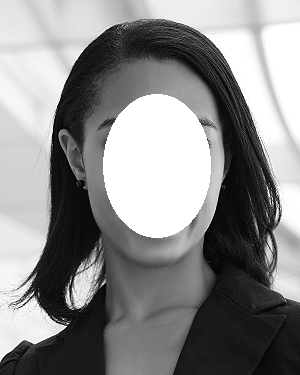
\includegraphics[width=1in,height=1.25in,clip,keepaspectratio]{author2.png}}]{Second B. Author} (M'76--SM'81--F'87) and all authors may include
biographies. Biographies are often not included in conference-related
papers. This author became a Member (M) of IEEE in 1976, a Senior
Member (SM) in 1981, and a Fellow (F) in 1987. The first paragraph may
contain a place and/or date of birth (list place, then date). Next,
the author's educational background is listed. The degrees should be
listed with type of degree in what field, which institution, city,
state, and country, and year the degree was earned. The author's major
field of study should be lower-cased.

The second paragraph uses the pronoun of the person (he or she) and not the
author's last name. It lists military and work experience, including summer
and fellowship jobs. Job titles are capitalized. The current job must have a
location; previous positions may be listed
without one. Information concerning previous publications may be included.
Try not to list more than three books or published articles. The format for
listing publishers of a book within the biography is: title of book
(publisher name, year) similar to a reference. Current and previous research
interests end the paragraph.

The third paragraph begins with the author's
title and last name (e.g., Dr.\ Smith, Prof.\ Jones, Mr.\ Kajor, Ms.\ Hunter).
List any memberships in professional societies other than the IEEE. Finally,
list any awards and work for IEEE committees and publications. If a
photograph is provided, it should be of good quality, and
professional-looking. Following are two examples of an author's biography.
\end{IEEEbiography}

\newpage

%If you do not have or do not want to include a photo, you can use IEEEbiographynophoto as shown below:

\begin{IEEEbiographynophoto}{Third C. Author, Jr.} (M'87) received the B.S. degree in mechanical
engineering from National Chung Cheng University, Chiayi, Taiwan, in 2004
and the M.S. degree in mechanical engineering from National Tsing Hua
University, Hsinchu, Taiwan, in 2006. He is currently pursuing the Ph.D.
degree in mechanical engineering at Texas A{\&}M University, College
Station, TX, USA.

From 2008 to 2009, he was a Research Assistant with the Institute of
Physics, Academia Sinica, Tapei, Taiwan. His research interest includes the
development of surface processing and biological/medical treatment
techniques using nonthermal atmospheric pressure plasmas, fundamental study
of plasma sources, and fabrication of micro- or nanostructured surfaces.

Mr. Author's awards and honors include the Frew Fellowship (Australian
Academy of Science), the I. I. Rabi Prize (APS), the European Frequency and
Time Forum Award, the Carl Zeiss Research Award, the William F. Meggers
Award and the Adolph Lomb Medal (OSA).
\end{IEEEbiographynophoto}

\EOD

\end{document}
